\section{Background}
Superconducting quantum computation with the advantage of sufficiently high controllability and low noise is a leading approach in the quantum computing competition.
Many groups including IBM,Google,and Riggetti choose it as a candidate for implementing medium and large-scale quantum computation.
In the paper, our architecture is designed for controlling superconducting quantum chip.
\subsection{control}

\begin{figure}[ht]
  \centering
  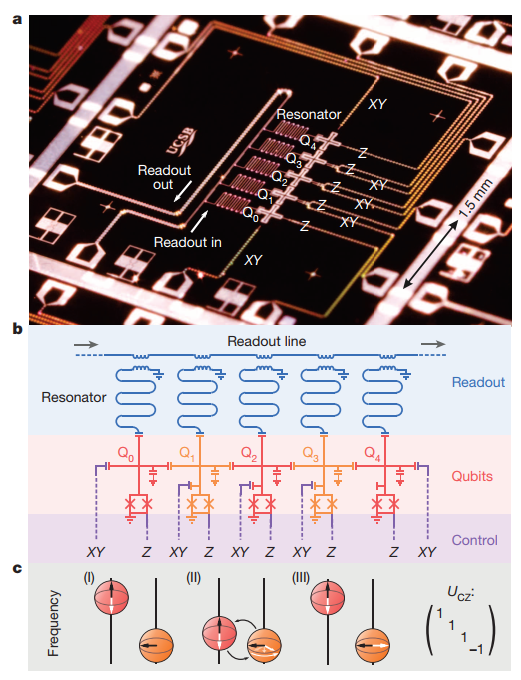
\includegraphics[width=\linewidth]{figure/background}
  \caption{ The quantum circuit based on the gate model and physical implementation}
  \label{imgb}
\end{figure}

Because we focus on how to control quantum chip, not the complex physical processes, 
we abstract quantum chip to an analog circuit and simplify the control problem to a simple process that apply a specific waveform to a specific control line at a specific time.



\ref{imgb} shows the connectivity of qubits and control lines. 
XY lines transfer pulsed microwaves produced by mixing two DAC outputs with a programmable local oscillator. When on resonance with the qubit, XY pulses 
will drive rabi oscillations which can be used to do single qubit gates. 
Z lines transfer static or dynamic voltages which can be used to tune the frequency of qubit and implement two qubit gates by flux biasing the SQUID. 
Readout line transfer pulsed microwaves which are similar to XY lines, but it has two ports that one for waveform input and one for waveform readout. 
When Readout-in waveform is on resonance with resonator, Readout-out waveform will contain status information of qubit.
In this structure, applying a single-qubit operation(like X,Y,H) on qubit is equivalent to apply a set pulsed microwaves on corresponding XY line. 
And similarly, applying a two-qubit operation(like Control-Z) on qubit is to apply a square wave on corresponding Z line.

\subsection{crosstalk}
Because of mutual and self-induction between Z lines, there is crosstalk in the flux biases of two qubits, where flux bias applied to one 
qubit can unintentionally induce flux in other qubits. 
Crosstalk can be regarded as leakage of the control signal and will corrupt the quantum state and lead to incorrect program execution.

For two qubits, crosstalk is expressed in terms of a 2x2 matrix M below.
\[ \begin{bmatrix} Z^r_1 \\ Z^r_2\end{bmatrix}=
\begin{bmatrix} M_1 & m_{12} \\ m_{21}  & M_2 \end{bmatrix} 
\begin{bmatrix} Z_1 \\ Z_2 \end{bmatrix}\]

Where $Z^r_1  $($Z^r_2 $) is the real flux biases of qubit1(qubit2), $Z_1  $($Z_2 $) is the intended flux biases we apply on qubits.In crosstalk matrix, $M_1=M_2=1 $, 
and $m_{12} $ and $m_{21} $ are the crosstalk terms, which are generally not equal to each other.by measuring the frequency change of qubit1(qubit2) with the variation 
of qubit1 Z-pulse and qubit2-Z pluse, We can get the crosstalk matrix.

And then, we can use the crosstalk matrix to make compensation of Z-pulses for reducing the effect of crosstalk.
According to the formula below, $Z_1  $($Z_2 $), the real flux biases needed to apply on Z line, will be inferred from the ideal flux biases $Z_1^{ideal}  $($Z_2^{ideal}  $).
\[\begin{bmatrix} Z_1 \\ Z_2\end{bmatrix}=
{\begin{bmatrix} M_1 & m_{12} \\ m_{21}  & M_2 \end{bmatrix}}^{-1}
\begin{bmatrix} Z_1^{ideal} \\ Z_2^{ideal} \end{bmatrix}\]

It means that the compensation Z-pulses for orthonormalize the control should be applied to all qubits even though we 
only do Z-control on one qubit if consider the effect of crosstalk.